\documentclass[12pt]{article}
\usepackage[utf8]{inputenc}
\usepackage{geometry}
\usepackage{multicol}
\usepackage{graphicx}
\usepackage{listings}
\geometry{margin=1in}

\title{Aritmética de punto flotante en Python}
\author{Rafael Villca Poggian\\Luis Alejandro Illanes Pinto}
\date{20/03/18}

\lstdefinestyle{mystyle}{
    basicstyle=\small,
    breakatwhitespace=false,         
    breaklines=true,                 
    captionpos=b,                    
    keepspaces=true,                 
    numbers=none,                    
    numbersep=5pt,                  
    showspaces=false,                
    showstringspaces=false,
    showtabs=false,                  
    tabsize=2
}
 
\lstset{style=mystyle}

\begin{document}

\maketitle
\graphicspath{ {/home/rafael/Desktop/Codes/Analisis_Numerico/art/} }
Dado que los números reales no se pueden codificar con número de bits, Python y la mayoría de los demás entornos informáticos técnicos usan “aritmética de punto flotante”, que implica un conjunto de infinitos números con precisión infinita. Esto conduce a los fenómenos de roundoff, underflow y overflow. La mayoría de las veces, es posible usar Python efectivamente sin preocuparse por estos detalles, sobre todo porque llegado a un punto empieza a usar cadenas para representar los n\'umeros, sacrificando tiempo por precisi\'on, pero, de vez en cuando, vale la pena saber algo sobre las propiedades y limitaciones de los números en punto flotante.
Antes de 1985, la situación era mucho más complicada de lo que es hoy. Cada computadora tenía su propio sistema numérico de punto flotante. Algunos eran binarios; algunos eran decimales. Hubo incluso una computadora rusa que usaba aritmética trinaría. Entre las computadoras binarias, algunas utilizan el 2 como la base; otros usaban 8 o 16. Y todos tenían una precisión diferente. En 1985, el IEEE, La Junta de Normas y el Instituto Nacional de Estándares Americanos adoptaron el ANSI / IEEE Estándar 754-1985 para aritmética binaria de punto flotante. Esta fue la culminación de casi una década de trabajo de un grupo de trabajo de 92 personas compuesto por matemáticos, informáticos e ingenieros de universidades, fabricantes de computadoras y compañías de microprocesadores.
Todas las computadoras diseñadas desde 1985 usan IEEE aritmética de punto flotante. Esto no significa que todos obtienen exactamente los mismos resultados, porque hay algo de flexibilidad dentro del estándar. Pero sí significa que ahora tenemos un modelo de máquina independiente de la aritmética del punto flotante y cómo se comporta. 
Python ha utilizado tradicionalmente el formato de precisión doble IEEE. Hay un solo formato de precisión que ahorra espacio, pero que no es mucho más rápido en las máquinas modernas. Abajo trataremos exclusivamente con doble precisión. También hay un formato de precisión extendida, que es opcional y por lo tanto es una de las razones de la falta de uniformidad entre diferentes máquinas.
La mayoría de los números de punto flotante distintos de cero están normalizados. Esto significa que pueden ser expresados como:
$$x = \pm{(1+f)}*2^e$$
El valor de f es la fracción o mantisa y “e” es el exponente. La fracción satisface:
$$0 \leq{f} < 1$$
Y debe ser representable en binario usando como máximo 52 bits. En otras palabras, $2^{52}f$ es un número entero en el intervalo:
$$0 \leq{2^{52}*f} < 2^{52}$$
El exponente e es un número entero en el intervalo:
$$-1022 \leq{e} < 1023$$
La finitud de f es una limitación de precisión. La finitud de e es una limitación en el rango.
Cualquier número que no cumpla con estas limitaciones debe ser aproximado por los que sí lo hacen.
Los números de punto flotante de doble precisión se almacenan en una palabra de 64 bits, con 52 bits para f, 11 bits para e, y 1 bit para el signo del número. El signo de e se acomoda almacenando e + 1023, que está entre 1 y $2^{11}$ -2. Los 2 valores extremos para el campo exponente, 0 y $2^{11}$ -1, están reservados para números excepcionales de punto flotante que describiremos más adelante.
La parte fraccionaria completa de un número de punto flotante no es $f$, sino $1 + f$, que tiene 53 bits. Sin embargo, el primer 1 no necesita ser almacenado. En efecto, el formato IEEE incluye 65 bits de información en una palabra de 64 bits.
El programa floatgui muestra la distribución de los números positivos en un sistema modelo
de punto flotante con parámetros variables. El parámetro t especifica la cantidad de bits
utilizados para almacenar $f$. En otras palabras, $2 ^ tf$ es un número entero. Los parámetros
$e_{min}$ y $e_{max}$ especifican el rango del exponente, entonces $e_{min} \leq{e} < e_{max}$. Inicialmente,
floatgui establece t = 3, $e_{min}$ = -4 y $e_{max}$ = 2 y produce la distribución que se muestra en la
figura 1.7.
\begin{center}
  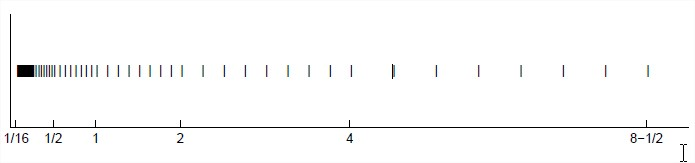
\includegraphics[scale=0.65]{fig1}
  FIGURA 1: Floatgui
\end{center}
Dentro de cada intervalo binario $2^e \leq{x} < 2^{e+1}$, los números están igualmente espaciados
con un incremento de $2^{e-t}$. Si e = 0 y t = 3, por ejemplo, el espaciado de los números
entre 1 y 2 es 1/8. A medida que $e$ aumenta, el espaciado aumenta.También es instructivo mostrar los números del punto flotante con una escala logarítmica. La
Figura 1.8 muestra floatgui con logscale comprobada y $t$ = 5, $e_{min}$ = -4 y $e_{max}$ = 3. Con esta
escala logarítmica, es más evidente que la distribución en cada intervalo binario es la misma.
Una cantidad muy importante asociada con la aritmética del punto flotante se resalta en rojo
por floatgui. Python llama a esta cantidad epsilon, contenida en la librer\'ia \textbf{sys}.
\begin{center}
epsilon es la distancia desde 1 hasta el siguiente número mayor de punto de coma flotante.
\end{center}
Para el modelo floatgui sistema de punto flotante, epsilon = $2^{-t}$.
Antes del estándar de la IEEE, las diferentes máquinas tenían diferentes valores de epsilon. Ahora,para doble precisión de la IEEE.
\begin{center}
  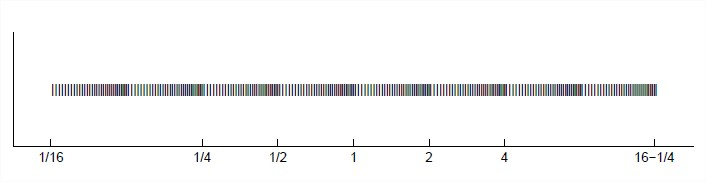
\includegraphics[scale=0.65]{fig2}
  FIGURA 2: Floatgui(escala logar\'itmica)\\
\end{center}
\lstinputlisting[language=Python]
{eps.py}
El valor decimal aproximado de eps es $2.2204*10^{-16}$. O bien eps/2 o eps se pueden
llamar el nivel de redondeo. El error relativo máximo incurrido cuando el resultado de una
operación aritmética se redondea al número de punto flotante más cercano es eps/2. El
espaciado relativo máximo entre números es eps. En cualquier caso, puede decir que el nivel
de roundoff es de aproximadamente 16 dígitos decimales.
Un ejemplo frecuente de roundoff ocurre con la simple declaración de Python:
\lstinputlisting[language=Python]
{t.py}
El valor matemático t almacenado en t no es exactamente 0.1 porque expresar la fracción
decimal 1/10 en binario que requiere una serie infinita. De hecho.
$$\frac{1}{10} = \frac{1}{2^4} + \frac{1}{2^5} + \frac{0}{2^6} + \frac{0}{2^7} + \frac{1}{2^8} + \frac{1}{2^9} + \frac{1}{2^{10}} + \frac{0}{2^{11}}+ \frac{1}{2^{12}}+ ...$$
Después del primer término, la secuencia de coeficientes 1, 0, 0, 1 se repite infinitamente a
menudo. Agrupar los términos resultantes juntos cuatro a la vez expresa 1/10 en una serie
base 16 o hexadecimal.
$$\frac{1}{10} = 2^{-4}*(1+\frac{9}{16}+\frac{9}{16^2}+\frac{9}{16^2}+\frac{9}{16^3}+\frac{9}{16^4}+...)$$
Los números de punto flotante en cualquier lado de 1/10 se obtienen al terminar la parte
fraccional de esta serie después de 52 términos binarios o 13 términos hexadecimales, y
redondeando el último término hacia arriba o hacia abajo. Así
$$t_1 < \frac{1}{10} < t_2$$
donde:
$$t_1 = 2^{-4}*(1+\frac{9}{16}+\frac{9}{16^2}+\frac{9}{16^3}+...+\frac{9}{16^{12}}+\frac{9}{16^{13}}),$$
$$t_1 = 2^{-4}*(1+\frac{9}{16}+\frac{9}{16^2}+\frac{9}{16^3}+...+\frac{9}{16^{12}}+\frac{9}{16^{13}}).$$
Resulta que 1/10 está más cerca de t2 que de t1, por lo que t es igual a t2. En otras palabras,
$$t = (1+f)2^e$$
d\'onde:
$$f = \frac{9}{16}+\frac{9}{16^2}+\frac{9}{16^3}+...+\frac{9}{16^{12}}+\frac{9}{16^{13}},$$
$$e = -4.$$
La funci\'on que escribimos en python para convertir a hexadecimal usando la librer\'ia struct:
\lstinputlisting[language=Python]
{double_to_hex.py}
hace que $t$ se muestre como:\\\\
$t: 3fb999999999999a$\\\\
Los caracteres a hasta f representan los "dígitos" hexadecimales del 10 al 15. Los primeros
tres caracteres, 3fb, dan la representación hexadecimal del decimal 1019, que es el valor del
exponente sesgado e + 1023 si e es -4. Los otros 13 caracteres son la representación
hexadecimal de la fracción f.
En resumen, el valor almacenado en t es muy cercano, pero no exactamente igual a 0.1. La
distinción es ocasionalmente importante. Por ejemplo, la cantidad\\\\
$0.3/0.1$\\\\
No es exactamente igual a 3 porque el numerador real es un poco menos de 0.3 y el
denominador real es un poco mayor que 0.1.
Diez pasos de longitud t no son exactamente lo mismo que un paso de longitud 1.\\
¿A qué se parece la aproximación de punto flotante a la proporción áurea?
\lstinputlisting[language=Python]
{phi.py}
produciendo:\\\\
$phi: 3ff9e3779b97f4a8$\\\\
El primer dígito hexadecimal, 3, es 0011 en binario. El primer bit es el signo del número de
punto flotante; 0 es positivo, 1 es negativo. Entonces phi es positivo. Los bits restantes de los
primeros tres dígitos hexadecimales contienen e + 1023. En este ejemplo, 3ff en la base 16
es $3*16^2 + 15*16 + 15 = 1023$ en decimal. Así que.
$$e = 0$$
De hecho, cualquier número de punto flotante entre 1.0 y 2.0 tiene e = 0, por lo que su salida
hexadecimal comienza con 3ff. Los otros 13 dígitos hexadecimales contienen f. En este
ejemplo:
$$f = \frac{9}{16}+\frac{14}{16^2}+\frac{3}{16^3}+...+\frac{10}{16^{12}}+\frac{8}{16^{13}},$$
con estos valores de $f$ y $e$:
$$(1+f)2^e \approx \phi$$
Otro ejemplo vendr\'ia a ser:
\lstinputlisting[language=Python]
{code.py}
con computaci\'on exacta, $e$ vendr\'ia a ser 0. Pero con punto flotante, la salida es la siguiente:\\\\
$a: 1.3333333333333333$\\
$b: 0.33333333333333326$\\
$c: 0.9999999999999998$\\
$e: 2.220446049250313e-16$\\\\
Resulta que el único redondeo ocurre en la división en la primera declaración. El cociente no
puede ser exactamente 4/3, excepto en esa computadora trinaria rusa. En consecuencia, el
valor almacenado en a es cercano, pero no exactamente igual a, 4/3. La resta b = a - 1
produce a b cuyo último bit es 0. Esto significa que la multiplicación 3 * b puede realizarse sin
ningún redondeo. El valor almacenado en c no es exactamente igual a 1, por lo que el valor
almacenado en e no es 0. Antes del estándar IEEE, este código se usó como una forma
rápida de estimar el nivel de redondeo en varias computadoras.\\
El nivel de redondeo eps a veces se llama “punto flotante cero" pero ese es un nombre
inapropiado.Hay muchos números de punto de coma mucho más pequeños que eps. El número más
pequeño de punto flotante normalizada positiva tiene f = 0 y e = -1022. El número de punto
flotante más grande tiene f un poco menos de 1 y e = 1023. la librer\'ia num\'erica por excelencia de Python, \textbf{numpy}, llama a estos números
tiny y realmax.\\
Junto con eps, caracterizan el sistema estándar.
\begin{center}
  \begin{tabular}{c c c}
    & Binario & Decimal\\
    eps & 2**(-52) & $202204e^{-16}$\\
    realmin & 2**(-1022) & $2.2251e^{-308}$\\
    realmax & (2 - eps)*2**1023 & $1.7977e^{+308}$
  \end{tabular}
\end{center}
Si cualquier cálculo intenta producir un valor mayor que realmax, se dice que es más lento.
El resultado es un valor excepcional de punto flotante llamado infinidad o Inf. Se representa
tomando e = 1024 y f = 0 y satisface relaciones como 1 / Inf = 0 e Inf + Inf = Inf.
Si cualquier cálculo intenta producir un valor que no está definido incluso en el sistema de
números reales, el resultado es un valor excepcional conocido como No-un-Número, o NaN.
Los ejemplos incluyen 0/0 e Inf-Inf. NaN se representa tomando e = 1024 y f distinto de cero.
Si cualquier cálculo intenta producir un valor más pequeño que realmin, se dice que es
underflow. Esto implica uno de los aspectos opcionales y controvertidos del estándar IEEE.
Muchas máquinas, pero no todas, permiten números excepcionales denormal o subnormal
de punto flotante en el intervalo entre realmin y eps * realmin. El número subnormal inferior
más pequeño es de aproximadamente 0.494e-323. Cualquier resultado más pequeño que
esto se establece en 0. En máquinas sin subnormales, cualquier resultado menor que
realmin se establece en 0. Los números subnormales llenan el espacio que se puede ver en
el sistema modelo floatgui entre 0 y el número positivo más pequeño. Proporcionan una
manera elegante de manejar underflow, pero su importancia práctica para el cálculo al estilo
de Python es muy raro. Los números denormales se representan tomando e = -1023, por lo
que el exponente sesgado e + 1023 es 0.
Python usa el sistema de punto flotante para manejar enteros. Matemáticamente, los
números 3 y 3.0 son los mismos, pero muchos lenguajes de programación usarían
representaciones diferentes para los dos. Python si distingue entre ellos. A veces usamos el
término pedernal para describir un número de coma flotante cuyo valor es un número entero.
Las operaciones de punto flotante en pedernales no introducen ningún error de redondeo,
siempre que los resultados no sean demasiado grandes. La suma, la resta y la multiplicación
de pedernales producen el resultado int exacto si no es más grande que $2^{53}$. La división y la
raíz cuadrada con pedernales también producen un int si el resultado es un número entero.\\
Una funci\'on de Python que descompone los n\'umeros de punto flotante es:\\\\

frexp\\\\

produce\\\\

print(help(frexp))\\\\
Help on built-in function frexp in module math:\\\\
frexp(...)\\
    frexp(x)\\\\    
    Return the mantissa and exponent of x, as pair (m, e).\\
    m is a float and e is an int, such that x = m * 2.**e.\\
    If x is 0, m and e are both 0.  Else 0.5 <= abs(m) < 1.0.\\\\
None\\\\

Adem\'as implementamos una funci\'on para restaurar el n\'umero descompuesto:
\lstinputlisting[language=Python]
{pow2.py}
Las cantidades F y E utilizadas por log2 y pow2 son anteriores al estándar de punto flotante de la IEEE y por lo tanto son ligeramente diferentes de las f y e que estamos usando en esta
sección. De hecho, f = 2 * F-1 y e = E-1.
\lstinputlisting[language=Python]
{descomponer_componer.py}
produce:\\\\
$F: 0.8090169943749475$\\
$E: 1$\\
$phi: 1.618033988749895$\\\\
Como ejemplo de cómo el error de redondeo afecta los cálculos de la matriz, considere el
conjunto 2 por 2 de ecuaciones lineales.
$$17x_1+5x_2=22$$
$$1.7x_1+0.5x_2=2.2$$
La solución obvia es $x_1 = 1$, $x_2 = 1$. Pero las declaraciones de Python:
\lstinputlisting[language=Python]
{eq1.py}
produce\\\\
$[[-1.25490196]$\\
$[8.66666667]]$\\\\
¿De dónde viene esto? Bueno, las ecuaciones son singulares, pero consistentes. La
segunda ecuación es solo 0.1 veces la primera. La x calculada es una de infinitamente
muchas soluciones posibles. Pero la representación en coma flotante de la matriz A no es
exactamente singular porque A[1,0] no es exactamente 17/10.El proceso de solución resta un múltiplo de la primera ecuación del segundo. El multiplicador
es mu = 1.7 / 17, que resulta ser el número de punto flotante obtenido al truncar, en lugar de
redondear, la expansión binaria de 1/10. La matriz A y el lado derecho b son modificados por:
\lstinputlisting[language=Python]
{eq2.py}
Con el cálculo exacto, tanto A[1,1] como b[1] se convertirían en cero, pero con la aritmética
de coma flotante, ambos se convierten en múltiplos de eps distintos de cero.\\\\
\textbf{A[1,1]=(1/4)*eps:} 5.55111512313e-17 = 5.551115123125783e-17\\\\
\textbf{b[1]=2*eps:} [  4.44089210e-16] = 4.440892098500626e-16\\\\
Python nota el pequeño valor de la nueva A[1,1] y muestra un mensaje que advierte que la
matriz está cerca del singular. Luego calcula la solución de la segunda ecuación modificada
dividiendo un error de redondeo por otro.\\\\
\textbf{x[1]=b[1]/A[1,1]:} [ 8.66666667] = [ 8.]\\\\
Este valor se sustituye de nuevo en la primera ecuación para dar\\\\
\textbf{x[0]=(22 - 5*x[1])/17:} [-1.25490196] = [-1.25490196]\\\\
Los detalles del error de redondeo llevan a \textbf{numpy} de Python a elegir una solución particular entre las
infinitas soluciones posibles para el sistema singular. Nuestro último ejemplo traza un
polinomio de séptimo grado.
\lstinputlisting[language=Python]
{grafica.py}
La gráfica resultante en la Figura 1.9 no se parece en nada a un polinomio. No es suave. Se puede observar un error de redondeo en acción. El factor de escala del eje $y$ es minúsculo, $10^{-14}$.
Los pequeños valores de $y$ se calculan tomando sumas y diferencias de números tan
grandes como $35*1.012^4$. Hay una cancelación sustractiva severa.\\\\
\begin{center}
  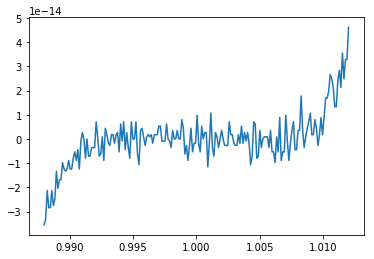
\includegraphics[scale=1]{grafica}\\
  FIGURA 3: Figura 1.9. Esto es un polinomio?\\
\end{center}
Si los valores de $y$ se calculan con:\\\\
y = (x-1)**7\\\\
se obitiene una gr\'afica muy suave.
\section*{Referencias}
\begin{enumerate}
\item Floating-Point Arithmetic in Matlab
\item Cleve Moler, Numerical Computing with MATLAB, SIAM, Philadelphia, 2004.
\end{enumerate}
\end{document}